\documentclass[12pt]{article}

\usepackage{float}
\usepackage[pdftex]{graphicx} 
\graphicspath{{../img/}}
\DeclareGraphicsExtensions{.pdf,.jpeg,.png,.jpg} 

\usepackage{listings}
\lstset{language=Python, keywordstyle=\color{blue}, stringstyle=\color{olive}, breaklines=true, showstringspaces=false, float, tabsize=2}
\usepackage{xcolor}
\usepackage{textcomp}
\usepackage{subcaption}
\usepackage{amsmath}
\newcommand{\source}[1]{\caption*{Source: {#1}} }
%opening
\title{Laboratory exercise no. 6: Simulation of stress and strain distribution using finite element method
}
\author{Piotr Gawry\'s $<pgawrys2@gmail.com>$}

\begin{document}

\maketitle

\section{Introduction}
The goal of this laboratory is to implement simulation of stress and strain distribution using finite element method. In contrary to earlier classes the simulation is not written entirely in code but it also takes advantage of MATLAB's Partial Differential Equation Toolbox.

\subsection{Mathematical Model}
\label{model}
Although the main goal is to conduct simulation without implementing equation manually we still want to calculate it and compare results with theoretical model. If the simulation object is cantilevered beam under a load then it will be deformed by a value \textbf{h} which can be calculated using formula below:

\begin{equation}
h = \frac{F \cdot L^3}{3E \cdot J}
\end{equation}
Where:
\begin{itemize}
	\item $F = 1000$ N -- loading force.
	\item $L = 1.5$ m -- beam length.
	\item $E = 1.8 * 10^{8}$ Pa -- Young's modulus.
	\item $J$ -- moment of inertia of plane area.
\end{itemize}

\begin{equation}
 J = \frac{g \cdot d^3}{12}
\end{equation}
Where:
\begin{itemize}
	\item $g = 1$ m -- beam thickness.
	\item $d = 0.2$ m -- beam width.
\end{itemize}


\section{Simulation}

The modelled object is cantilevered beam supported from the left side. In this simulation we will explore situation where some force is applied at the end (right side) going downwards.

\begin{figure}[H]
	\centering
	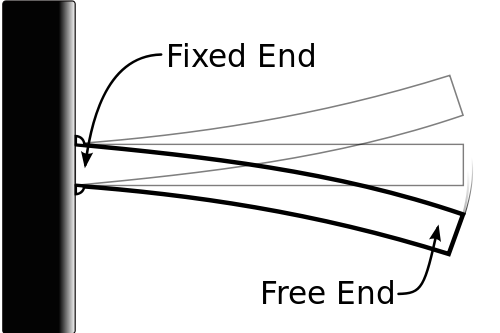
\includegraphics[width=\textwidth]{2}
	\caption{Cantilever Beam.}
	\source{https://commons.wikimedia.org/wiki/File:Cantilever\_Beam.svg}
	\label{2}
\end{figure}
 
\subsection{PDE Toolbox}
To implement simulation we will use \textbf{pdetool} (included in Partial Differential Equation Toolbox) which provides an interactive for solving 2-D geometry problems. Running it is as simple as writing \textit{pdetool} in MATLAB's Command Window.

\subsection{Drawing the object}

After turning on Options $\rightarrow$ Grid and selecting Draw $\rightarrow$ Rectangle/square we can draw simulated object using parameters described in the previous section which are 0.2 m for width and 1.5 m for length. This is reflected in the rectangle's dimensions.

\begin{figure}[H]
	\centering
	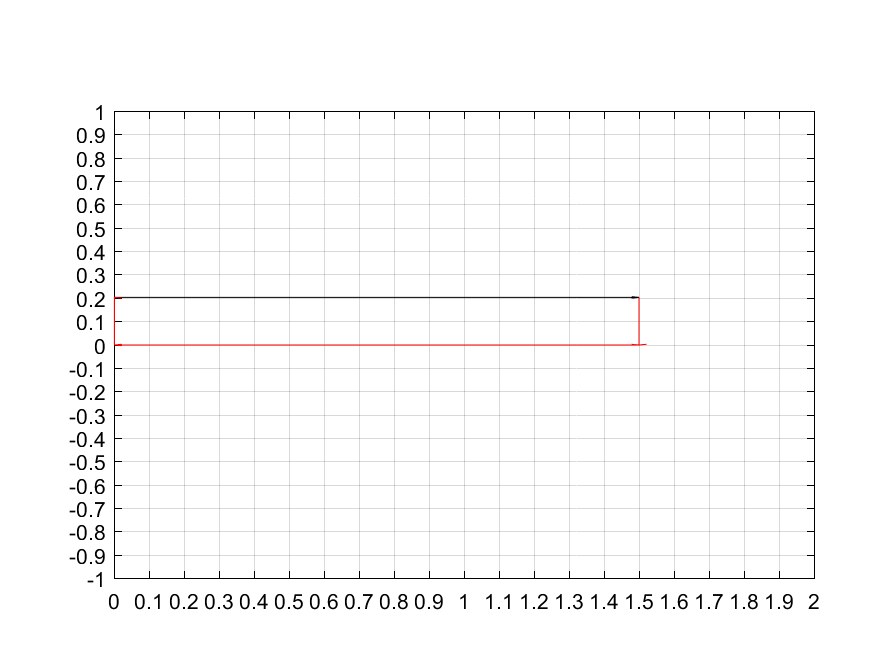
\includegraphics[width=\textwidth]{1}
	\caption{Cantilever Beam drew using MATLAB's PDE Toolbox in boundary mode.}
	\label{1}
\end{figure}

\subsection{Setting boundary conditions}

To correctly define model we need to include boundary conditions taking into account beam support (left side) and force load (top right side going downwards).

First of all we need to choose correct type of PDE application in the drop down at the top -- for our uses \textit{Structural Mech, Plane Strain} works fine. Next, entering boundary mode is done choosing Boundary $\rightarrow$ Boundary Mode or clicking Ctrl + B with default setup. Clicking any side twice causes Boundary Condition window to pop up. We are using following parameters:

\begin{enumerate}
	\item Left -- h11 = 1, h12 = 0, h21 = 0, h22 = 1
	\item Top -- h11 = 0, h12 = 0, h21 = 0, h22 = 0
	\item Right -- g1 = 0, g2 = -1000 (with Neumann condition)
	\item Bottom -- h11 = 0, h12 = 0, h21 = 0, h22 = 0
\end{enumerate}

Note that values for \textbf{Left} indicate that this side won't move under pressure (since it is supported). 

g2 = -1000 indicates 1000 N applied downwards.

\subsection{Coefficients in the equation}

After setting boundary conditions we should set coefficients in PDE $\rightarrow$ PDE Specification. According to https://www.engineeringtoolbox.com, Young's modulus for Stainless Steel is about 1.8E8 Pa, Poisson's ratio is 0.305 and density is between 7480 - 8000 $\frac{kg}{m^3}$. For the purpose of the simulation middle value was chosen (7740 $\frac{kg}{m^3}$).

\begin{figure}[H]
	\centering
	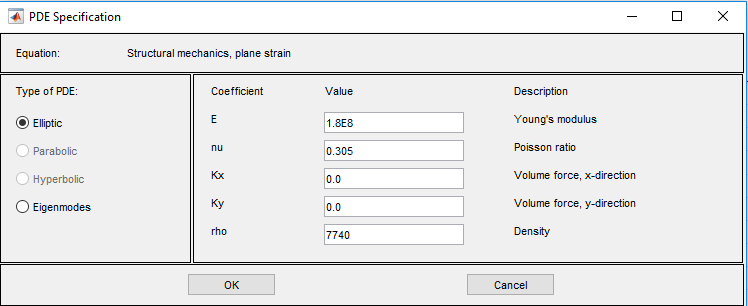
\includegraphics[width=\textwidth]{3}
	\caption{PDE specification with entered variables.}
\end{figure}

\subsection{Visualization}

Final steps are to calculate and visualize simulation. Mesh $\rightarrow$ Mesh Mode and then Mesh $\rightarrow$ Refine Mesh followed by Solve $\rightarrow$ Solve PDE is all it takes to prepare model for visualization.

In Plot $\rightarrow$ Parameters... there are various options for plotting the result. Most interesting for this use case is changing \textbf{Property} to \textbf{y displacement (v)}. The plot is shown in the figure ~\ref{4}.

\begin{figure}[H]
	\centering
	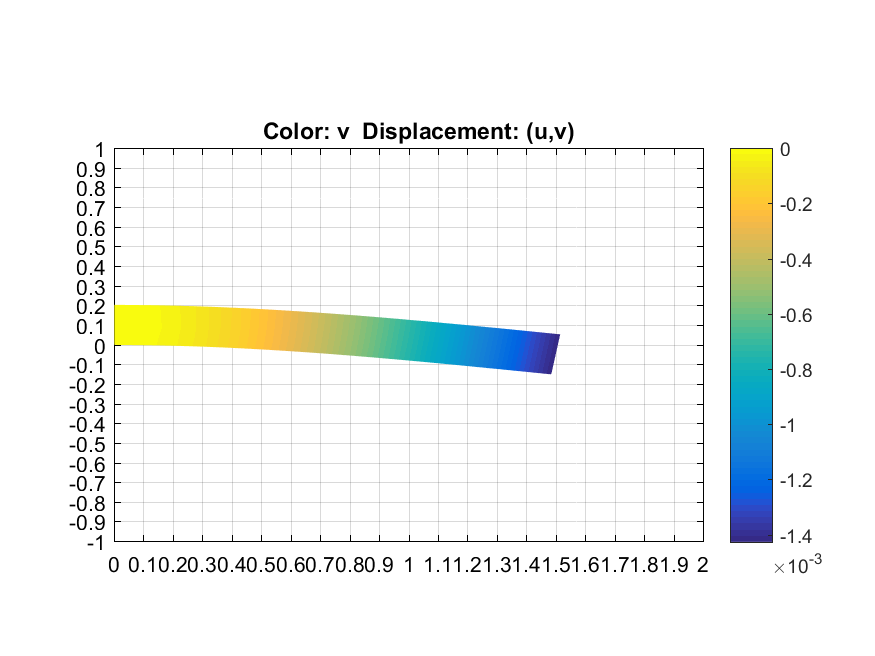
\includegraphics[width=\textwidth]{4}
	\caption{Cantilever Beam after 1000 N pressure from the right side visualized using PDE Toolbox.}
	\label{4}
\end{figure}

We don't observe any deformation on the left side because beam is attached but there is a significant deformation closer to the point of applied force.

It is possible to know the exact values of deformation by exporting solution (Solve $\rightarrow$ Export Solution) to MATLAB. It returns an array with -0.0014 as lowest value which is consistent with the plot (dark blue color is -0.0014). That's a good point to compare with manual approach.

\subsection{Comparison to theoretical model}
Relevant equations were introduced in section ~\ref{model}. We could either calculate it by hand or using MATLAB, implementation is straightforward:
\lstinputlisting[language=Matlab,frame=single]{../source_code/calc.m}

The value \textbf{h} at the very end (right side) is \textbf{-0.0094} which means almost 7 times higher deformation than result obtained from using PDE Toolbox (\textbf{-0.0014}). It stays within the same order of magnitude but it's noticeable difference nonetheless. Perhaps it is caused by more sophisticated machinery behind PDE Modeler (due to possibility of taking into account additional parameters about stainless steel such as density which were not present in used equation) leading to more accurate result or just human error.

\subsection{More complicated geometry}
Cantilever beam is just a rectangle which might not be convincing use case for PDE Toolbox since it can be calculated by hand without too much effort. Fortunately, nothing is stopping us from drawing much more complicated shapes.

Figures ~\ref{elo} present schematics and solved plot for a bit more complicated shape attached in two places, less regular width and different forces.

Implementing this in code would be more educating process but also much slower -- entire process of this simulation took minutes.


\begin{figure}[H]
	\centering
	\begin{subfigure}[b]{0.8\textwidth}   
		\centering 
		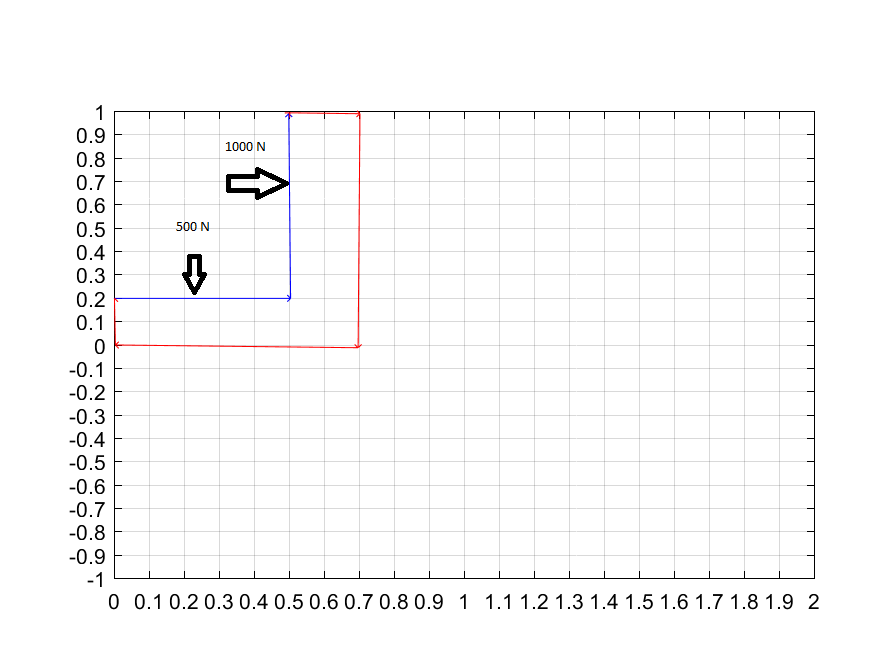
\includegraphics[width=\textwidth]{5}  
	\end{subfigure}
	\begin{subfigure}[b]{0.8\textwidth}   
		\centering 
		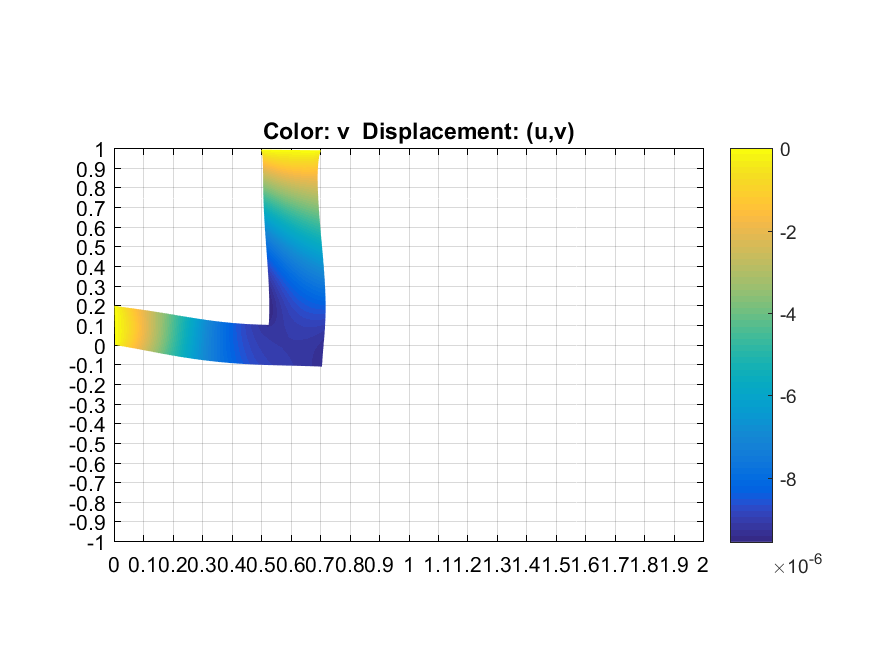
\includegraphics[width=\textwidth]{6}
	\end{subfigure}
\caption{L-shaped stainless steel Beam attached from the left and top with 1000 N applied at left side of the top arm and 500 N on top side of the bottom arm.}
\label{elo}
\end{figure}

\section{Conclusion}

Over the course of this classes we learned how to simulate stress and strain simulation using PDE Toolbox. Although manual calculations can give us better understanding and confidence about given model the PDE Toolbox is very easy to use and allows for fast prototyping with nice visualization.

I can easily imagine very complicated shapes which are insanely hard to implement and maintain using pure code so I would say using such toolbox scales better for more complicated problems and whenever we have doubts about precision of modelling simulation we can work with generated code to search for issues.

\end{document}
